%!TEX root = ../../Systementwurf2.tex

\section{Implementierung von Komponente <C20>: Webinterface}

Das Webinterface stellt eine Schnittstelle für Benutzer und Administratoren bereit, in dem sie ihre Einstellungen verwalten können. Es wird mit dem Play-Framework implementiert und kommuniziert mit dem Server eventbasiert mittels Akka.

\subsection{Paket-/Klassendiagramm}

\begin{figure}[ht]
\centering
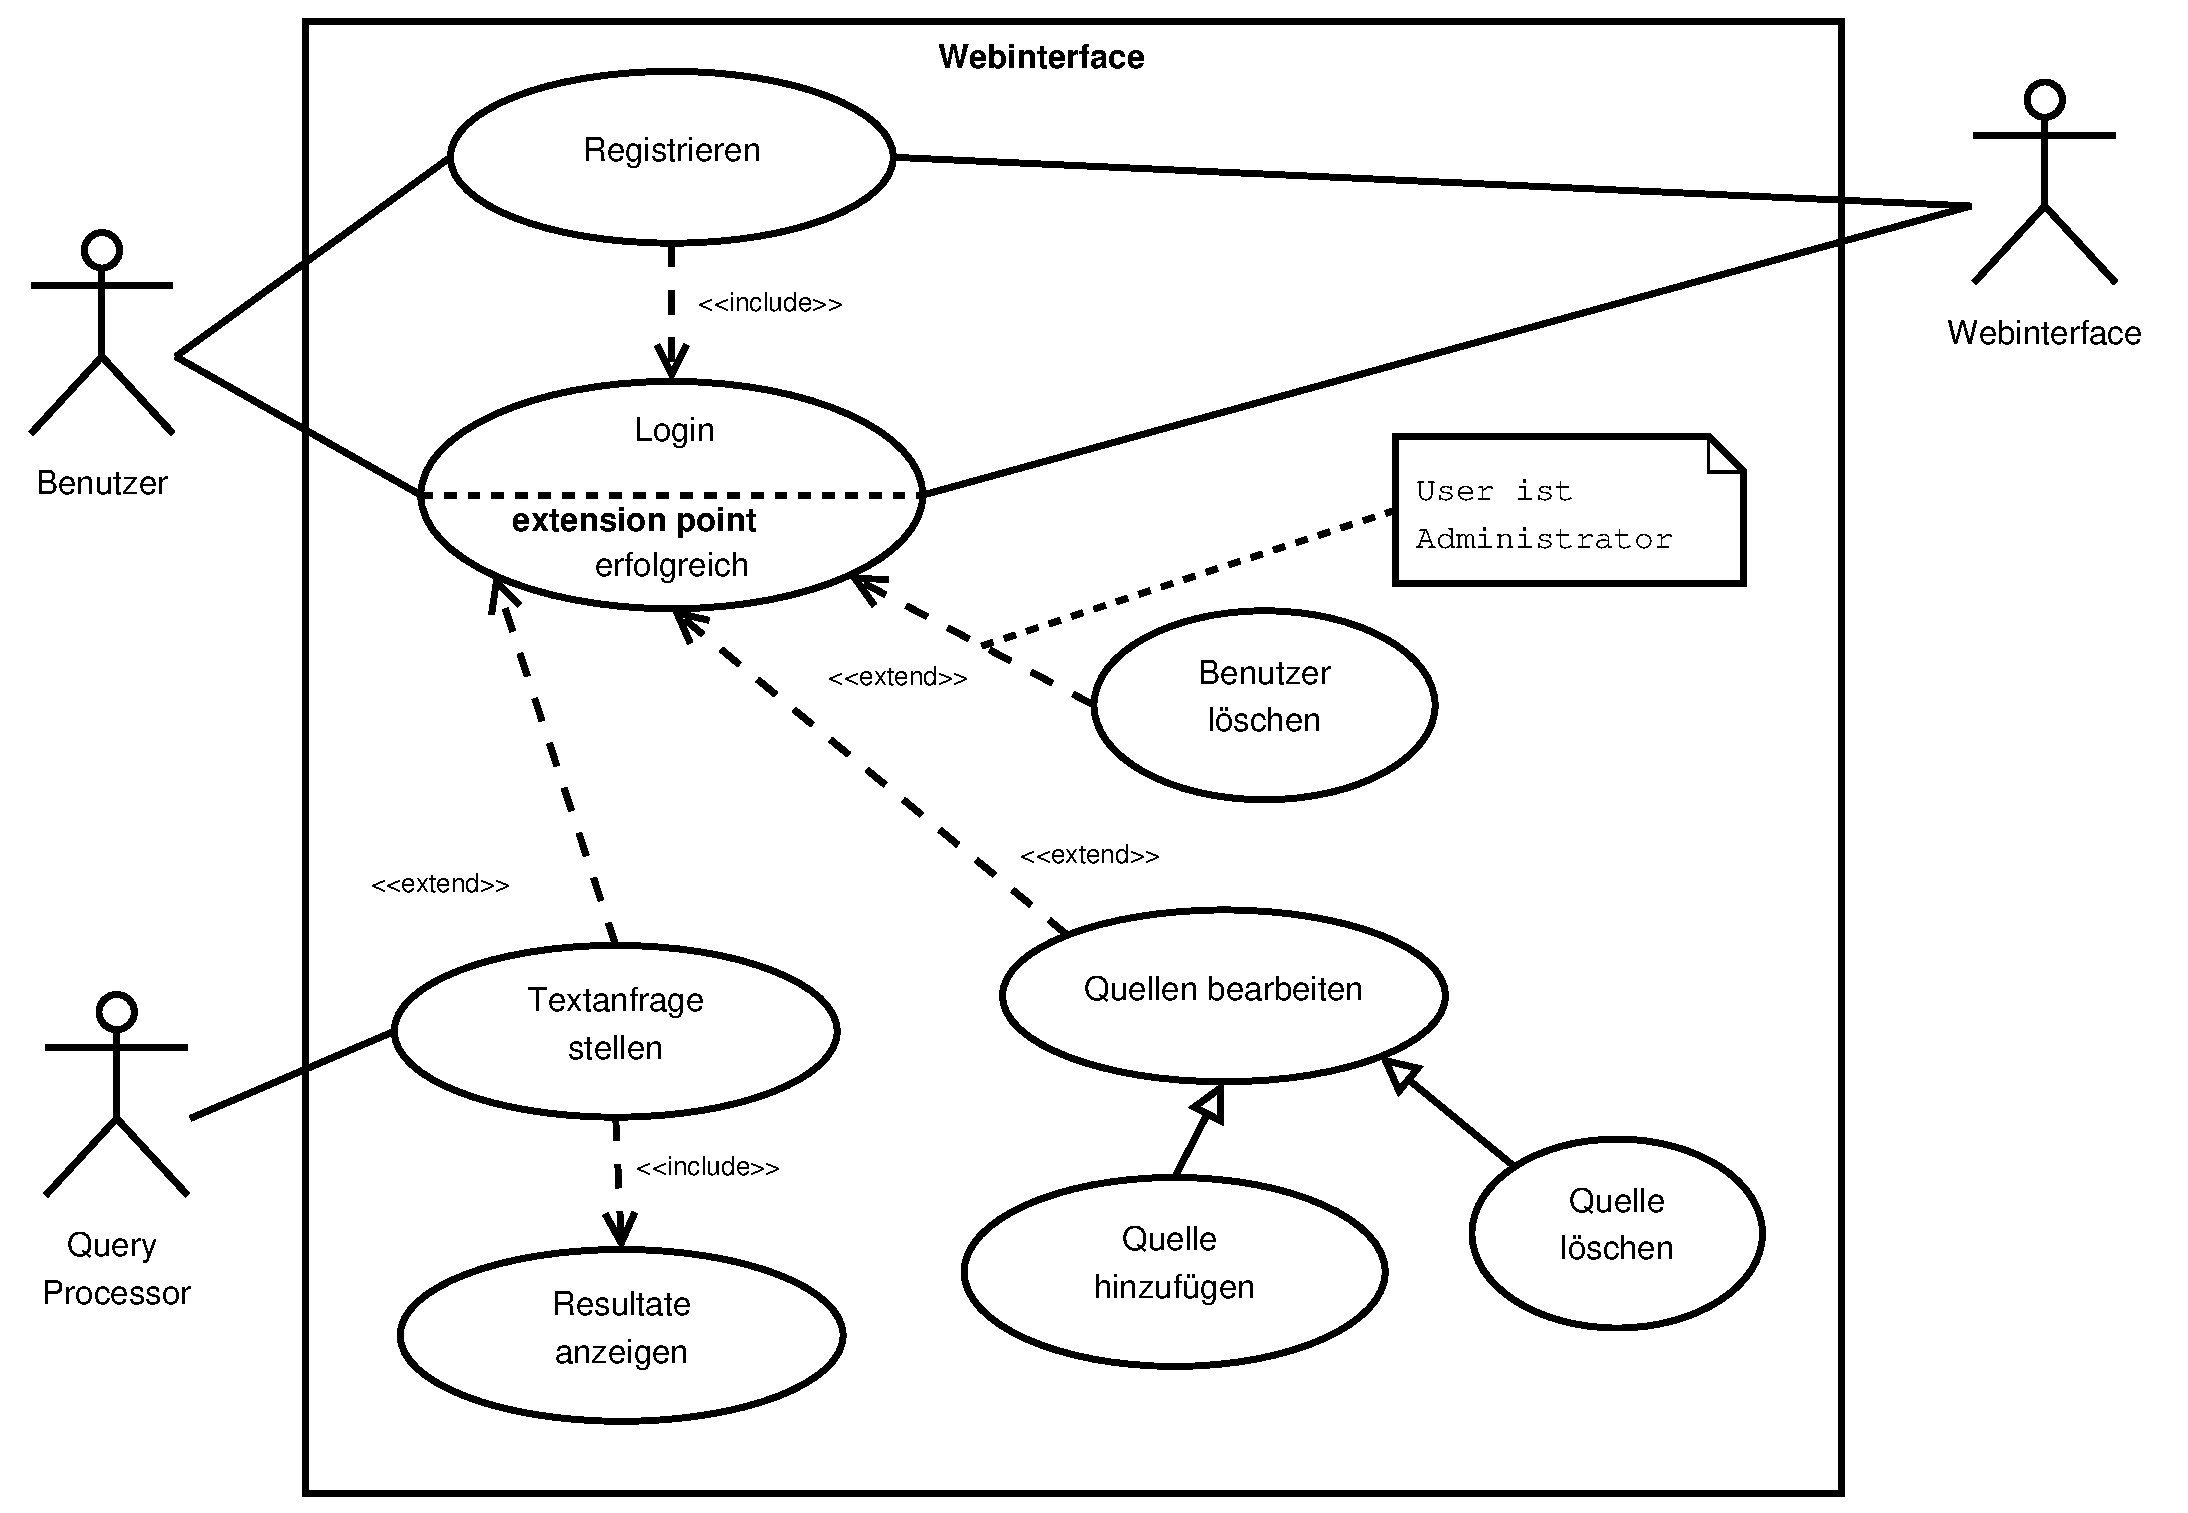
\includegraphics[width=1.03\textwidth]{Systementwurf/05_implementierungsentwurf/webinterface}
\caption{Klassendiagramm für Komponente \ref{C20}}
\end{figure}

\subsection{Erläuterung}

Im Folgenden werden Attribute, Aufgaben und Kommunikationspartner für jede Klasse des Webinterfaces kurz erläutert.\\
Die Funktionen der Klassen (außer Communication) besitzen keine Parameter, da diese per HTTP übertragen werden.

\begin{class}{10}{Communication}
\item[Aufgabe]~\
Die Communication-Klasse ist für die Kommunikation mit dem Server zuständig.
\item[Attribute]~\ keine
\item[Operationen]~\
\begin{itemize}
  \item \texttt{loginRequest(String, String)}: Sendet eine Anfrage, um einen Benutzer einzuloggen.
  \item \texttt{registerRequest(String, String, String)}: Sendet eine Anfrage, um einen neuen Benutzer zu registrieren.
  \item \texttt{userFeedsRequest(User)}: Sendet eine Anfrage, um alle Feeds eines Benutzers zu erhalten.
  \item \texttt{addFeedRequest(User, List<Feed>)}: Sendet eine Anfrage, um einen Benutzer mit Feeds zu verknüpfen.
  \item \texttt{removeFeedRequest(User, List<Feed>)}: Sendet eine Anfrage, um die Verknüpfungen zwischen einem Benutzer und Feeds zu entfernen.
  \item \texttt{userListRequest()}: Sendet eine Anfrage, um eine Liste aller Benutzer zu erhalten.
  \item \texttt{deleteUserRequest(User)}: Sendet eine Anfrage, um einen Benutzer zu löschen.
  \item \texttt{changeAdminRequest(User)}: Sendet eine Anfrage, um einem Benutzer Administratorenrechte zu gewähren oder zu entziehen.
  \item \texttt{createFeedRequest(Feed)}: Sendet eine Anfrage, um einen neuen Feed anzulegen.
  \item \texttt{deleteFeedRequest(Feed)}: Sendet eine Anfrage, um einen Feed zu löschen.
\end{itemize}
\item[Kommunikationspartner]~\
  \textit{ServerHandler}
\end{class}

\begin{class}{20}{AdminFeeds}
\item[Aufgabe]~\
Die AdminFeeds-Klasse stellt die Webseite zum Administrieren von Feeds zur Verfügung.
\item[Attribute]~\ keine
\item[Operationen]~\
\begin{itemize}
    \item \texttt{showFeedsControl()} Zeigt die Webseite an.
    \item \texttt{addFeed()} Sendet eine Anfrage, einen neuen Feed zu erstellen.
    \item \texttt{deleteFeed()} Sendet eine Anfrage, einen Feed zu löschen.
\end{itemize}
\item[Kommunikationspartner]~\ keine
\end{class}

\begin{class}{30}{AdminUser}
\item[Aufgabe]~\
Die AdminUser-Klasse stellt die Webseite zum Administrieren von Benutzern zur Verfügung.
\item[Attribute]~\ keine
\item[Operationen]~\
\begin{itemize}
    \item \texttt{showUserControl()} Zeigt die Webseite an.
    \item \texttt{userAction()} Löscht einen Benutzer oder ändert seinen Admin-Status.
\end{itemize}
\item[Kommunikationspartner]~\ keine
\end{class}

\begin{class}{40}{Settings}
\item[Aufgabe]~\
Die Settings-Klasse stellt die Webseite zum Ändern der Benutzereinstellungen zur Verfügung.
\item[Attribute]~\ keine
\item[Operationen]~\
\begin{itemize}
    \item \texttt{showSettings()} Zeigt die Webseite an.
    \item \texttt{changePassword()} Sendet eine Anfrage, das Passwort zu ändern.
    \item \texttt{changeLanguage()} Sendet eine Anfrage, die Sprache zu ändern.
\end{itemize}
\item[Kommunikationspartner]~\ keine
\end{class}

\begin{class}{50}{Query}
\item[Aufgabe]~\
Die Query-Klasse stellt die Webseite zum Stellen eines Text-Queries zur Verfügung.
\item[Attribute]~\ keine
\item[Operationen]~\
\begin{itemize}
    \item \texttt{showQueryl()} Zeigt die Webseite an.
    \item \texttt{runQuery()} Sendet eine Anfrage mit einem Text-Query.
\end{itemize}
\item[Kommunikationspartner]~\ keine
\end{class}

\begin{class}{60}{Feeds}
\item[Aufgabe]~\
Die Feeds-Klasse stellt die Webseite zum Verwalten der Feedeinstellungen zur Verfügung.
\item[Attribute]~\ keine
\item[Operationen]~\
\begin{itemize}
    \item \texttt{showFeedsl()} Zeigt die Webseite an.
    \item \texttt{subscribe()} Sendet eine Anfrage, Feeds zu abonnieren.
    \item \texttt{dleteFeed()} Sendet eine Anfrage, Feeds zu deabonnieren.
\end{itemize}
\item[Kommunikationspartner]~\ keine
\end{class}

\begin{class}{70}{Application}
\item[Aufgabe]~\
Die Application-Klasse stellt die Startwebseite zur Verfügung.
\item[Attribute]~\ keine
\item[Operationen]~\
\begin{itemize}
    \item \texttt{index()} Zeigt die Startseite an.
\end{itemize}
\item[Kommunikationspartner]~\ keine
\end{class}

\begin{class}{80}{Login}
\item[Aufgabe]~\
Die Login-Klasse stellt die Webseite zum Einloggen zur Verfügung.
\item[Attribute]~\ keine
\item[Operationen]~\
\begin{itemize}
    \item \texttt{showLogin()} Zeigt die Webseite an.
    \item \texttt{login()} Sendet eine Anfrage, einen Benutzer einzuloggen.
    \item \texttt{logout()} Sendet eine Anfrage, einen Benutzer auszuloggen.
\end{itemize}
\item[Kommunikationspartner]~\ keine
\end{class}

\begin{class}{90}{Register}
\item[Aufgabe]~\
Die Register-Klasse stellt die Webseite zum Registrieren zur Verfügung.
\item[Attribute]~\ keine
\item[Operationen]~\
\begin{itemize}
    \item \texttt{showRegister()} Zeigt die Webseite an.
    \item \texttt{register()} Sendet eine Anfrage, einen neuen Benutzer zu registrieren.
\end{itemize}
\item[Kommunikationspartner]~\ keine
\end{class}

\begin{class}{100}{Recovery}
\item[Aufgabe]~\
Die Recovery-Klasse stellt die Webseite zum Wiederherstellen des Passworts zur Verfügung.
\item[Attribute]~\ keine
\item[Operationen]~\
\begin{itemize}
    \item \texttt{showRecovery()} Zeigt die Webseite an.
    \item \texttt{recover()} Sendet eine Anfrage, das Passwort wiederherzustellen.
\end{itemize}
\item[Kommunikationspartner]~\ keine
\end{class}